\documentclass{acm_proc_article-sp}
\usepackage{graphicx}
\usepackage{float}
\usepackage{epstopdf}



\begin{document}

\title{A Comparison of Scheduling Algorithms}
\numberofauthors{1}
\author{
\alignauthor
Samuel Jackson\\
       \affaddr{Aberystwyth University}\\
       \email{slj11@aber.ac.uk}
}
\date{\today}

\maketitle
\begin{abstract}

\end{abstract}

% A category with the (minimum) three required fields
\category{D.4}{Operating Systems}{Process Management}[Scheduling]
%A category including the fourth, optional field follows...
\category{D.2.8}{Software Engineering}{Metrics}[complexity measures, performance measures]

\terms{Algorithms, Performance, Measurement}

\keywords{Algorithms, Scheduling, Performance, Lottery Scheduling, Shortest Time Remaining, Round Robin}

\section{Introduction}
This report aims to examine the differences between three approaches to scheduling algorithms that are widely used in systems throughout computer science where multiple tasks require computation in parallel. Scheduling algorithms are used to organise and prioritise jobs of computation according to a set scheme which deals with the issues such as throughput, turnaround and context switches.

The scheduling algorithms used here are Shortest Time Remaining (STR), round robin and lottery scheduling which were chosen because they all exhibit characteristics which make them suitable in different situations. The former two are deterministic in nature while lottery scheduling is non deterministic. STR takes a simple queue based approach, while round robin uses time slices to share processing time. Lottery scheduling uses probabilistic methods to give higher priority jobs a greater likelihood of being selected.

\section{Methodology} 
\label{methodology}
To thoroughly test the performance of the algorithms, each of the schedulers was exercised using a set of data files each of which test different properties important to scheduling algorithms. This includes files which contain a heavy amount of I/O processing, a low level of I/O processing, jobs where all priorities are the same, and some general test data. Test data that is heavy in I/O processes exercises how well an algorithm handles a high level of context switching due to jobs being blocked for reading or writing. The data file with a low level of I/O is used to evaluate the performance of the scheduler in situations which would not require I/O. A file where all priorities are the same is used to help evaluate lottery scheduling (which schedules according to priority) to evaluate its worst case performance.

Th method used to test each algorithm was to run it with each of the supplied generic data files and to also test it with the custom data files to evaluate how each algorithm handles specific aspects of scheduling. The results are then compared against one another using five attributes important to scheduling algorithms (mean duration, total CPU time, number of context switches, idle time and time for first job to finish) in order to show how each algorithm performed both with generic test data and specific test data to gain an idea of how well each performed both generally and within a specific area of performance.

Because lottery scheduling is non-deterministic it required a different approach to testing that involved an extra step. Lottery scheduling gives different results on each run, therefore in order to evaluate an average run an automated simulator was created to simulate 10,000 runs of the algorithm per test file. The results of this data could then be averaged out to representatively compare lottery scheduling's general case performance with the performance of the other algorithms.

\section{Results}
\label{results}
This section details the outcomes of testing each of the algorithms using the data files outlined in section \ref{methodology} to measure four key attributes important to scheduling algorithms. As mentioned in the preceding section, the values used with lottery scheduling are the mean results of 10,000 tests.

\subsection{Mean Duration}
\label{results-duration}
Mean duration is the average amount of time that a scheduled job takes to finish processing. Figure \ref{fig:duration} shows that the mean duration time across all tests and algorithms was fairly consistent, with Shortest Time Remaining (STR) having the lowest mean duration in all tests. Round Robin scheduling showed the worst performance of the four with means durations slight above those of FCFS and Lottery scheduling, both of whom presented mixed results depending on the test.

\begin{figure}[H]
\centering
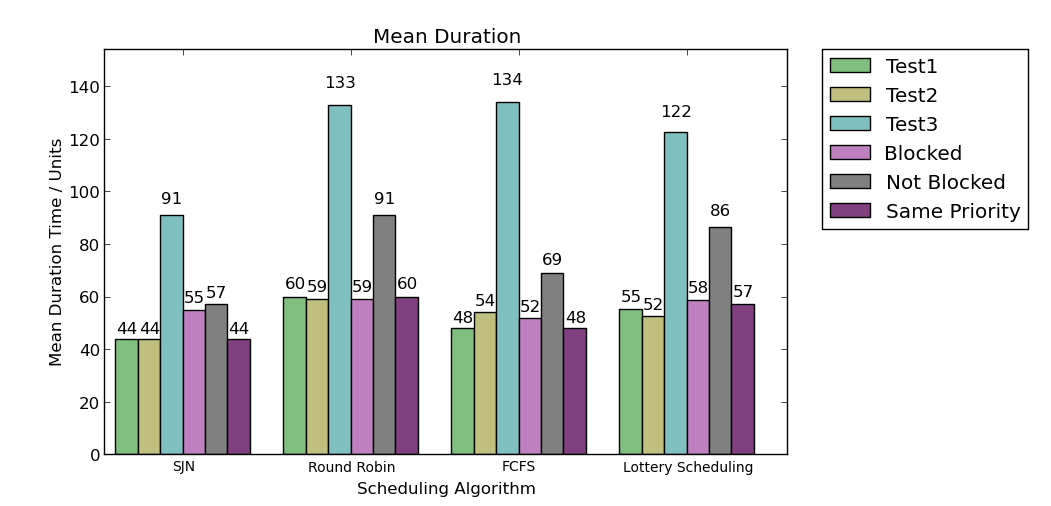
\includegraphics[width=0.5\textwidth]{duration.png}
\caption{Mean Job Duration across all tests and algorithms}
\label{fig:duration}
\end{figure}

The mean duration appears to spike on test 3 and on the test with no I/O blocking, although STR appeared to show a significantly lower mean duration time for the no I/O test than the other schedulers.

\subsection{CPU Time}
CPU time is the number of CPU ticks that each algorithm performs in total in order to complete all of the jobs. Figure \ref{fig:cpu-time} shows that the CPU times were also fairly consistent across all tests with Round Robin besting or equalling the other algorithms. Conversely, STR performed slightly worse in this criteria than the others. Also, FCFS exhibited a higher CPU time at 191 ticks as opposed to a consistent 182 ticks for every other algorithm. 

\begin{figure}[H]
\centering
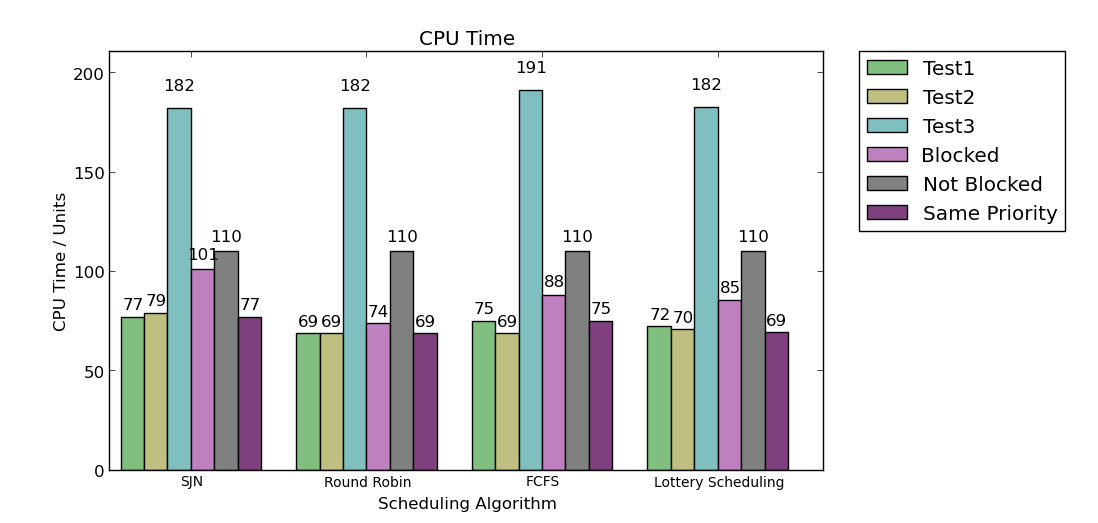
\includegraphics[width=0.5\textwidth]{cpu_time.png}
\caption{CPU time to complete processing jobs across all tests and algorithms.}
\label{fig:cpu-time}
\end{figure}

\subsection{Context Switches}
Context switches measure the number of times the algorithm switches between different jobs while executing them (if at all). Figure \ref{fig:ctex-switches} shows a mixed result between FCFS and STR in terms of the number context switches made with FCFS having the lowest result on tests 1,2, the high I/O blocking test and the test with all priorities the same and STR scoring lower on the other two tests. Round Robin had the worse performance overall with Lottery scheduling following closely behind. 

Interestingly, FCFS had a very high number of context switches on tests 3 and the non I/O blocking test when compared with its closest counterpart STR. In fact, the STR algorithm exhibited the lowest number of context switches in the non I/O blocking test. This is in sharp contrast with it giving the second highest number of context switches in all other algorithms.

\begin{figure}[H]
\centering
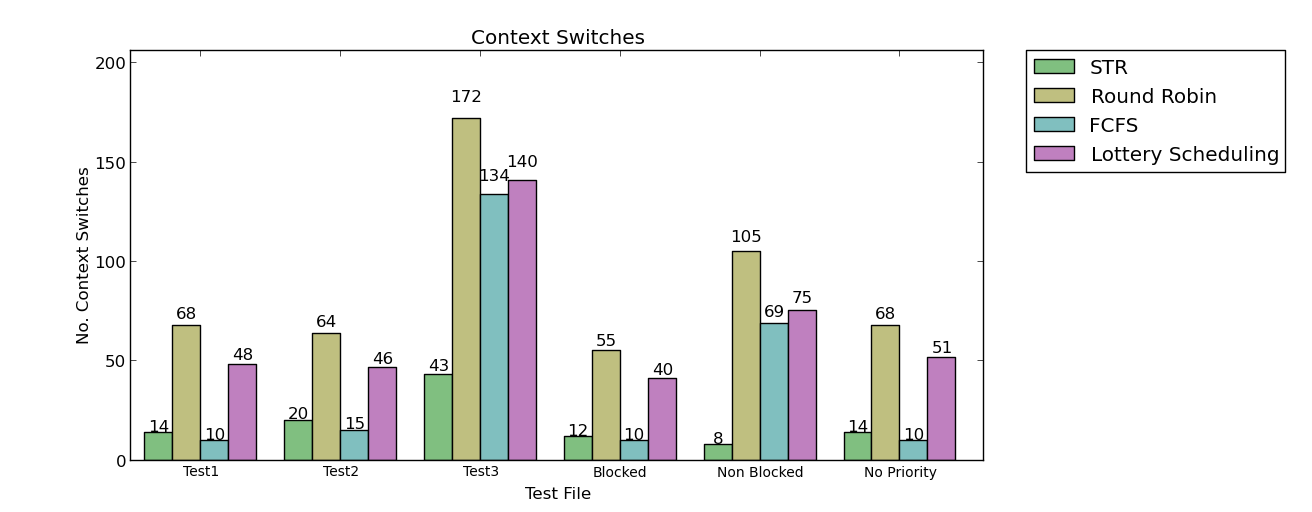
\includegraphics[width=0.5\textwidth]{ctex_switches.png}
\caption{Total number of context switches across all tests and algorithms.}
\label{fig:ctex-switches}
\end{figure}

\subsection{Idle Time}
Idle time is the number of CPU ticks that occur where there were no jobs pending within the scheduler as they were all either finished on blocked for I/O. Figure \ref{fig:idle-time} shows the total idle times for all tests as a percentage of the CPU time which clearly shows Round Robin to be the winner with only 5 idle cycles during the high I/O blocking test and 0 idle time for every other test. Lottery scheduling performed reasonably we, while STR and FCFS showed mixed results. Interestingly, STR had no idle time in test 3 while FCFS had no idle time in test 2. STR had a significantly higher idle time during the non blocking I/O test with 31.7\% of its CPU time spent idle. The high I/O blocking test proved to show the largest impact on the idle time compared with the other tests.

\begin{figure}[H]
\centering
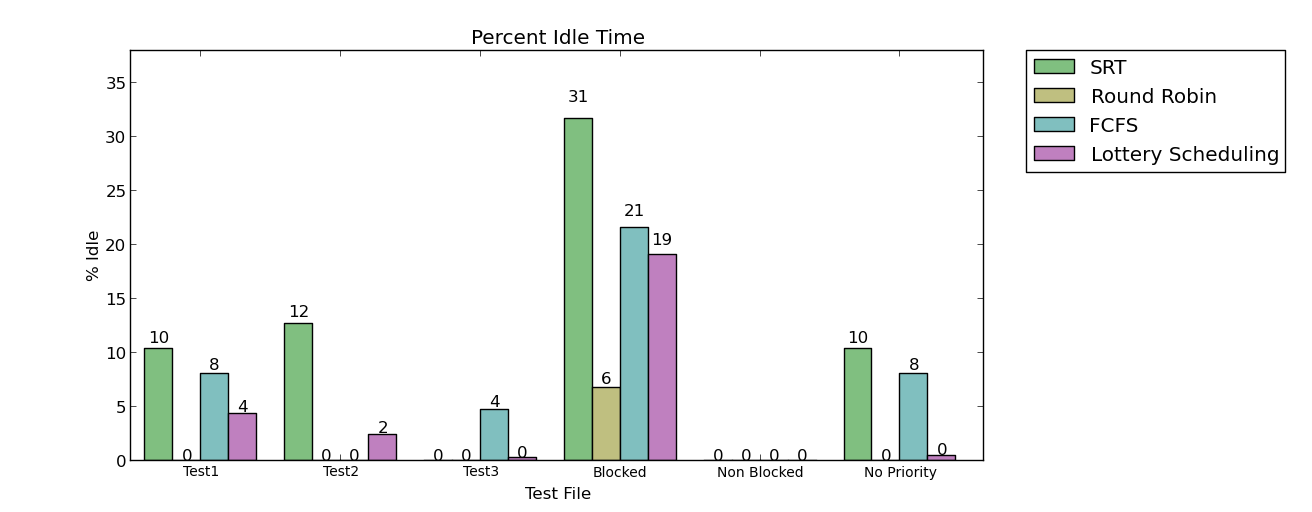
\includegraphics[width=0.5\textwidth]{idle_time_per.png}
\caption{Total idle time as a percentage of CPU time across all tests and algorithms.}
\label{fig:idle-time}
\end{figure}

\subsection{First Job Finish Time}
\label{results-fstjob-time}
This final section shows the time taken for the first job to finish across all tests. Figure \ref{fig:fstjob-time} clearly shows that STR to be significantly faster than both Round Robin and Lottery scheduling as well as being generally faster than FCFS. Round Robin has the slowest performance in this category, with test 3 taking 92 cycles in order to finish the first job compared to just 15 cycles using STR.

\begin{figure}[H]
\centering
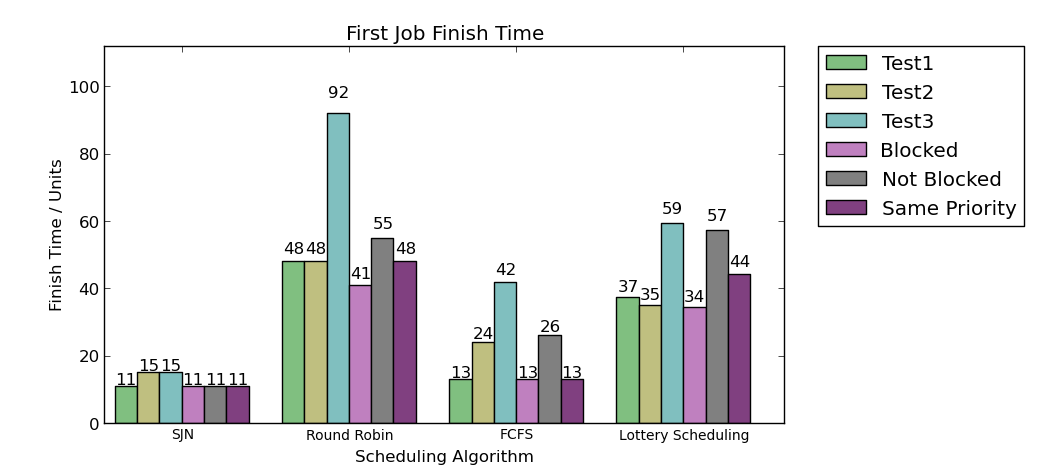
\includegraphics[width=0.5\textwidth]{fstjob_time.png}
\caption{Time for the first job to finish across all tests and algorithms.}
\label{fig:fstjob-time}
\end{figure}

\section{Discussion}
This section discusses the results presented in section \ref{results} to examine the strengths and weaknesses of each algorithm in each of the following categories: first job finish time, mean job finish time, and overall processing time.

\subsection{First Job Finish Time}
The results shown in subsection \ref{results-fstjob-time} clearly suggest that the Shortest Time Remaining algorithm is the fastest at finishing the first job. This seems logical because STR priorities new and returning jobs by the amount of processing that they ave left and therefore the STR will put the shortest jobs towards the start of the queue and longer jobs towards the back. This means that regardless of the test data, SJN puts the shortest job at the front and this job will get immediate processing and (providing it does require an I/O block, will finish in the shortest possible amount of time possible.

This is in contrast with the other three algorithms which do not order their jobs according to time remaining. Round Robin scheduling had the worst result in this category. Again, this seems logical because Robin Robin allocates equal CPU time slices to to each job regardless of its size or priority, suggesting that the shortest job will take much longer to finish as processing time must be shared equally between this job and the other jobs in the queue. The is confirmed by the data shown in figure \ref{fig:fstjob-time} where the first job in test 3 (by far the longest set of jobs) takes much more time to finish than in any other test. The slightly higher result for the test with no I/O blocking shows a higher finishing time for the first job. This is presumably because the less jobs that get blocked, the more jobs are in the queue and the longer a job must wait for more CPU time.

The first come, first served algorithm appeared to be the second best choice after STR with two thirds of the first job tests finishing with 10 cycles of STR. However, as with Round Robin, FCFS does not prioritises the shortest job, but rather accepts the first job added to the queue and and continues working on it until it finishes or if it becomes blocked for I/O, in which case it is returned to the back of the queue. Therefore the time taken for the first job to finish in FCFS depends upon two factors which are the size of first job in the queue and whether the job will become blocked for I/O. 

If the job becomes blocked for I/O then it will be added to the back of the queue and will have to wait for all of the processes in front of it to finish before it will get CPU time again. If there are lots of jobs that require being blocked for I/O (such as those shown in the high I/O blocking test) then FCFS will begin to cycle through jobs rather than concentrating on a single job until it's done.

Lottery scheduling appeared to come off as the average case in the results presented in subsection \ref{results-fstjob-time}. As with Round Robin and FCFS, the implementation of lottery scheduling used here does not prioritise jobs according to their length (although it could be implemented to prioritise by job length) but instead uses the priority assigned to be job inside the testing file (which is presumably a arbitrary number according to the current importance of the job on the system). Because jobs are weighted according to priority and not the size of the job, and because this implementation is pre-emptive, there is no guarantee about the length of time taken for the first job to finish. The speed that the initial job will finish in is decided by a jobs priority and random chance.

\subsection{Mean Job Duration Time}
When considering the mean time to finish a job, It appears that the Shortest Time Remaining algorithm proves to be the best option. Referring to Figure \ref{fig:duration} we can see that on average STR had the shortest mean time to finish a job compared with any other algorithm. This would appear to coincide with expectations as the STR algorithm always attempts to bring the shortest job to the front of the queue which mean they finish very quickly thus pulling the mean duration down. However, this comes with the caveat that longer processes can be starved of CPU time when there are lots of small jobs. This could be a particularly nasty problem if there is a constant stream of small jobs being added to the queue as this would force the mean duration to grow much higher as longer jobs would have to wait a long time.

The second best performing algorithm in this section was First Come, First Served which exhibited only slightly higher mean durations across all tests except in the case of test 3 where is was the worst performer and test 2 where it was narrowly beaten by lottery scheduling. Once again this seems to correlate with predictions. FCFS processes jobs as they arrive, so a queue with only a few short jobs will perform fairly similarly to STR. However, when are a lot of jobs on the queue the algorithms performance begins to deteriorate as longer processes begin to hold the CPU meaning shorter or higher priority jobs get starved of resources. Also, because of the lack of prioritisation, jobs that have been blocked are returned to be back of the queue regardless of the amount of processing left which means nearly complete tasks can be placed right at the back of the queue increasing their duration.

As for the other two tests, figure \ref{fig:duration} shows that Lottery scheduling came a narrow third with Round Robin coming in last. The reason for this is most likely because these two algorithms are more orientated around sharing CPU resources according to time or priority rather than attempting to gain maximum throughput like STR, making it a more appropriate choice when maximum throughput is not essential.

The data shown in \ref{fig:duration} shows that the difference in mean duration increases between the shorter tests (1 \& 2) and the longer test 3. Looking at the results shown in figure \ref{fig:fstjob-time} we can see that Round Robin had the highest first job finish time. These two points show that the mean duration is affected in Round Robin scheduling because the mean is altered due to jobs generally taking a longer time to finish than with the other scheduling algorithms. It is suggested that because jobs a cycled through in the order they are added, the shorter jobs are not finished as quickly as with other approaches as they are constantly waiting for time on the CPU and hence upping their duration and therefore the mean duration.

Finally, Lottery scheduling shares similar issues with Round Robin in the test of mean duration. Lottery scheduling has a higher mean duration that STR and FCFS because the its approach to scheduling uses randomness and the priority of the job (which has nothing to do with job size) to select which job should get processing time next. This means that, like Round Robin, shorter jobs may not be prioritised CPU time and therefore will generally take longer than with STR. However, unlike Round Robin, CPU is not shared equally among all jobs. This coupled with the element of randomness ensuring that all jobs are potentially allotted processing time makes the likely mean duration of Lottery scheduling difficult to quantify, but generally appears to be slightly quicker than with Round Robin in the average case, but because of Lottery scheduling being non-deterministic the performance may vary per run.

\subsection{Overall Processing Time}
When comparing the overall processing time taken to complete the tests as seen in figure \ref{fig:cpu-time}, Round Robin appears to be marginally better than the other algorithms where it either equals or surpasses every other scheduler in CPU time.

\section{Conclusions}

\section{Acknowledgements}
The author wishes to thank Richard Shipman (rcs@aber.ac.uk) for providing the supporting simulation code and GUI.

\bibliographystyle{abbrv}
\bibliography{sigproc}  % sigproc.bib is the name of the Bibliography 
\appendix
\subsection{References}
\balancecolumns
\end{document}